\documentclass[preprint,12pt,authoryear,doubleblind]{elsarticle}

\usepackage{amsmath}
\usepackage{booktabs}
\usepackage{graphicx}
\usepackage{threeparttable}
\usepackage{lineno}
\usepackage{url}
\usepackage{microtype}

\journal{Journal of Transport Geography}
\biboptions{authoryear,round}
\graphicspath{{./}{../figures/}}

\begin{document}
\begin{frontmatter}

\title{Reliability or continuity? How measurement changes the geography of New York subway elevator service}

% Blinded manuscript for double-anonymized review: author information intentionally omitted.

\begin{abstract}
Step-free rail access depends on more than the presence of elevators. It also depends on how continuously those assets remain available, and that continuity can look different when an operator excludes parts of calendar time from its reliability denominator. We examine 46,400 elevator--month records for 420 New York City subway elevators across 133 station complexes from January 2015 to October 2026. The analysis compares Metropolitan Transportation Authority (MTA)-reported availability with calendar service continuity, which retains all calendar hours in the denominator. In 2025, systemwide MTA-reported availability was 97.61\%, while calendar continuity was 90.20\%; the gap reached 15.77 percentage points in the Bronx. The difference was spatially selective rather than uniform. Metric choice changed which station complexes appeared persistently low-reliability: Cortlandt Street was in the monthly lowest quartile in 13.3\% of valid months under MTA-reported availability and 67.3\% under calendar continuity. Relative station-complex rankings also persisted across years under both metrics. At borough scale, asset-level availability and the MTA's accessible-platform metric were correlated, yet their complete four-borough ordering matched in only 10.5\% of overlapping months. These results show that the denominator of an operational reliability indicator can alter the geography of step-free infrastructure monitoring. Calendar continuity therefore complements conditional availability when the analytical task is to identify where prolonged service loss accumulates.
\end{abstract}

\begin{keyword}
Public transport \sep Accessibility \sep Reliability \sep Service continuity \sep Step-free access \sep Disability
\end{keyword}

\end{frontmatter}
\linenumbers

\section{Introduction}

Step-free rail access depends on both infrastructure provision and the continuity of the vertical links that make that infrastructure usable. A station can be classified as accessible while an elevator connecting the street, mezzanine, or platform is unavailable for part of the month. For travellers who cannot substitute stairs, elevator operation is therefore a basic service-side condition of step-free travel. This condition is especially visible in legacy rail systems, where accessible paths often depend on a limited number of vertical circulation assets.

Transport geography has long treated accessibility as a relationship between transport supply, spatial opportunities, and the constraints that shape travel \citep{geurs2004}. The updated accessibility framework also retains an explicit temporal component and recognises that different operationalisations can represent different aspects of accessibility \citep{geurs2026}. Recent work has shown how strongly measurement choices can shape spatial diagnosis. \citet{qu2025} found that the spatial resolution used to represent public transport access changes both the magnitude and geography of measurement error. \citet{schroth2026} similarly showed that an adjusted accessibility indicator can reveal over- and underserved areas that conventional measures do not identify. These studies make the construction of an indicator part of the analytical problem rather than a neutral technical step.

A related literature distinguishes scheduled transport supply from the service that is actually delivered. Real-time disruptions reduce realised accessibility relative to scheduled conditions \citep{liu2024}; recurring delays alter job-accessibility estimates \citep{nichols2024}; and travel-time variability can change measured accessibility inequalities \citep{braga2026}. For mobility-disabled travellers, operational reliability matters because the feasible network is already more constrained than for travellers able to use stairs or non-accessible alternatives \citep{liu2023}. Real-time elevator status has also been treated directly as an accessibility-information problem. \citet{sharif2022} collected elevator outage information across six North American rail systems and visualised whether nominally accessible stations were affected at a given time. That work demonstrates the practical importance of elevator operation. The question here is different: how does the definition of reliability change a long-run spatial diagnosis of elevator service?

New York City provides an unusually detailed case for examining that question. The Metropolitan Transportation Authority (MTA) publishes monthly equipment-level elevator availability over more than a decade. The published rate describes the share of reported service time during which an elevator is available. City accessibility reporting further notes that elevators undergoing planned replacement are excluded from the availability rate \citep{mopd2025}. This convention is well suited to evaluating equipment while it is counted as in service. It leaves a second monitoring question open: how much of the full calendar period is the asset recorded as available to provide elevator service?

That distinction matters geographically when excluded time is concentrated rather than evenly distributed. A systemwide availability rate can remain high while particular station complexes experience long periods outside the reported denominator. In that situation, changing the denominator can alter the relative ranking of places even when the published metric is internally consistent. Both indicators are internally valid; the question is whether they identify the same locations as persistently low-reliability.

This paper examines that problem using the New York City subway. Existing research has documented disability-related transit disparities \citep{liu2023}, realised accessibility losses under disruptions \citep{liu2024}, and additional travel burdens created by elevator placement within railway stations \citep{arai2026}. Open-data work has also represented New York subway vertical paths and elevator redundancy \citep{twosigma2020}. The present study stays at the asset and station-complex levels and isolates a prior measurement question: whether the temporal denominator used for elevator reliability changes the geography of long-run service-side monitoring.

Three research questions structure the analysis. First, how large and spatially variable is the gap between MTA-reported elevator availability and calendar service continuity? Second, does denominator choice change which station complexes are identified as persistently low-reliability locations, and are those relative rankings stable across years? Third, how closely does the asset-level geography correspond to the MTA's separate accessible-platform availability metric at borough scale?

These questions imply a simple spatial test. If denominator-excluded time is distributed proportionally across the subway system, calendar continuity should mainly shift the level of the indicator while preserving the ranking of places. If excluded time clusters in particular station complexes, the alternative denominator should change relative rankings and the set of locations repeatedly identified as low-reliability. The analysis therefore focuses on spatial reclassification and longitudinal rank persistence rather than the citywide mean alone.

The contribution is a measurement framework with a spatial consequence for transport geography. Calendar continuity complements MTA-reported availability by retaining calendar time that is absent from the operator's reliability denominator. Comparing the two reveals when an apparently technical denominator choice changes place-based monitoring. The resulting service geography is not a passenger-accessibility measure by itself. It is a service-side input that can be linked to path redundancy, passenger exposure, or population characteristics in subsequent accessibility and equity analyses.

\section{Operational reliability and step-free infrastructure}

\subsection{From nominal provision to service continuity}

Accessibility measures are selective representations of transport systems. Their usefulness depends on whether their assumptions match the decision problem being studied \citep{geurs2004}. In public transport, scheduled service provides a reproducible baseline, yet realised conditions can diverge substantially. \citet{liu2024} distinguished scheduled accessibility from accessibility under disruptions, while \citet{nichols2024} showed that recurring delays reduce realised access to employment in geographically uneven ways. \citet{braga2026} further demonstrated that incorporating travel-time variability can change the scale of measured inequality.

The same measurement logic applies to vertical access infrastructure. A binary indicator that a station contains an elevator describes provision, but it does not describe the time dimension of service. Transit performance guidance has long treated elevator reliability as an operational performance measure whose interpretation depends on service time and maintenance records \citep{tcrp2003}. An equipment availability percentage is therefore meaningful only in relation to the denominator used to define exposure. When long replacement or capital-work periods are excluded, the resulting percentage describes conditional in-service reliability. A calendar-time denominator answers a different question about continuity over the full month.

For step-free travel, the asset metric captures one service-side layer. Passenger accessibility also depends on path redundancy: one unavailable elevator may remove the only feasible vertical link at one station while remaining redundant at another. Research on mobility disabilities shows that formal transit provision and actual use can differ substantially \citep{liu2023}. Recent railway research likewise shows that elevator placement can impose additional travel-time burdens even at stations that are formally accessible \citep{arai2026}. Elevator service continuity therefore represents one layer of a broader accessibility system.

\subsection{Why the geography of reliability matters}

A systemwide average can conceal persistent local service loss. If particular station complexes repeatedly occupy the lower tail of the reliability distribution, the pattern is spatially structured rather than a sequence of isolated failures. That structure matters because a place that repeatedly experiences low continuity warrants different diagnosis from a systemwide random outage risk.

Recent JTG research increasingly treats transport reliability as a spatial problem. Recurring delays produce geographically differentiated accessibility losses \citep{nichols2024}; disruptions affect the reliability of delivered accessibility \citep{liu2024}; and service variability interacts with urban structure to change measured inequality \citep{braga2026}. Related work separates service-side signals from opportunity-side disadvantage because different indicators can identify different spatial regimes \citep{kang2026}. Elevator data allow that logic to be examined at the infrastructure layer: the question is whether the vertical assets that support step-free movement provide continuous service in the same places over time.

New York is particularly useful because the MTA provides a long monthly equipment panel together with a separate borough-level accessible-platform indicator. These sources allow the measurement gap to be examined at system, borough, and station-complex scales, while the platform indicator provides an independent higher-level comparison of spatial ordering.

\section{Data and methods}

\subsection{Data}

The primary source is the MTA NYCT Subway Elevator and Escalator Availability dataset \citep{mta_availability2026}. We use the version downloaded on 16 November 2026. After filtering to elevators, the analytical file contains 46,400 equipment--month observations representing 420 elevators at 133 station complexes between January 2015 and October 2026. The equipment--month key contains no duplicates. The data include equipment identifiers, station and station-complex identifiers, borough, management responsibility, outage counts, hours available, reported total hours, and the published 24-hour availability rate.

We verified the published percentage directly. For every observation with a positive reported denominator,
\begin{equation}
A_{it} = \frac{H^{\mathrm{avail}}_{it}}{H^{\mathrm{reported}}_{it}},
\end{equation}
where $A_{it}$ is the published 24-hour availability for elevator $i$ in month $t$. The reconstructed value matches the published field to numerical precision.

The second source is the MTA Subway Accessible Station Platform Availability dataset \citep{mta_platform2026}. It reports, by month and borough from 2018 onward, the percentage of time that the average accessible platform is available to passengers requiring step-free access. The uploaded snapshot contains 525 borough--month observations. We use the four subway boroughs---Bronx, Brooklyn, Manhattan, and Queens---for comparison with the elevator data.

Station-complex coordinates used for mapping were obtained from the MTA station reference data and aggregated to the complex level. The spatial analysis is restricted to complexes with sufficient longitudinal coverage for chronicity assessment.

\subsection{Reported availability and calendar service continuity}

The central methodological distinction concerns the denominator. The published availability measure uses hours included in the MTA's reported service denominator. We construct a second measure using the total number of hours in the calendar month:
\begin{equation}
C_{it} = \frac{H^{\mathrm{avail}}_{it}}{H^{\mathrm{calendar}}_{t}},
\end{equation}
where $H^{\mathrm{calendar}}_{t}$ equals 24 times the number of days in month $t$.

We call $C_{it}$ \emph{calendar service continuity}. It is deliberately not labelled ``true availability''. The two metrics address different questions. $A_{it}$ measures reliability conditional on the operator's reported denominator; $C_{it}$ measures the share of the calendar month during which the asset is recorded as available. Their difference is
\begin{equation}
G_{it} = A_{it} - C_{it}.
\end{equation}
A positive $G_{it}$ indicates time that is absent from the reported availability denominator. This can include periods associated with major replacement or other excluded states. The MTA's public accessibility reporting confirms that planned replacement periods are excluded from the published elevator availability rate \citep{mopd2025}.

System, borough, and station-complex aggregates are hours-weighted. For a group $g$, we sum available hours and the relevant denominator before taking the ratio, rather than averaging percentages across assets.

\subsection{Spatial persistence and chronic disadvantage}

For each station complex and month, we calculate both reported availability and calendar continuity from the combined elevator hours at that complex. Within each month, station complexes are ranked separately by the two metrics. A complex is classified in the low-reliability quartile if it falls in the lowest 25\% of observed complexes for that month.

For each complex with at least 36 observed months, we then calculate the proportion of months spent in the lowest quartile under each metric. This converts one-off outages into a longitudinal measure of chronic disadvantage. The difference between the two recurrence shares measures reclassification caused by the denominator choice.

To test whether relative reliability is persistent through time, we aggregate reported availability by complex and year and calculate Spearman rank correlations between consecutive years. A persistent positive correlation means that places with relatively low reliability in one year also tend to rank relatively low in the next.

\subsection{Maintenance governance}

The dataset distinguishes elevators managed by NYCT from those managed by third parties. The sample contains 369 NYCT-managed elevators and 51 third-party-managed elevators. We estimate the association between management type and reported availability using
\begin{equation}
A_{it} = \beta T_i + \alpha_t + \gamma_s + \varepsilon_{it},
\end{equation}
where $T_i$ indicates third-party management, $\alpha_t$ are month fixed effects, and $\gamma_s$ are station-complex fixed effects. Standard errors are clustered by elevator. The complex fixed effects compare management types within the same broader station environment while month effects absorb system-wide temporal shocks.

Because management type is not randomly assigned, $\beta$ is interpreted as an association rather than a causal effect. As a sensitivity analysis, we repeat the model only for the 13 station complexes that contain observations from both management types.

\subsection{Cross-scale validation}

Finally, we examine whether equipment-level availability and the agency's accessible-platform availability metric provide the same spatial diagnosis. Elevator observations are aggregated to borough--month reported availability and merged with the official platform metric for the overlapping period. We report Pearson and Spearman correlations, mean absolute error, and the frequency with which the two metrics produce the same ordering of all four boroughs. The ranking comparison is important because transport-geographical interpretation often depends less on a citywide mean than on which places are identified as relatively better or worse served.

\subsection{Sensitivity checks}

Three checks address choices that could otherwise drive the calendar-continuity result mechanically. First, we decompose calendar service loss into two additive components: unavailable hours inside the MTA-reported denominator and hours excluded from that denominator. This shows whether the observed gap reflects ordinary outages or the treatment of excluded time. Second, we remove the first and last observed month of each elevator, reducing the possibility that partial installation or retirement months inflate calendar exposure. Third, we repeat the chronicity analysis using minimum longitudinal-coverage thresholds of 24, 36, 48, 60, and 72 months. A spatial reclassification is treated as robust when its direction and substantive threshold remain stable across these alternatives.


\section{Results}

\subsection{The measurement gap is large in some years and spatially uneven}

MTA-reported availability and calendar continuity are close in some years and widely separated in others (Fig.~\ref{fig:trend}). The systemwide gap was 0.39 percentage points in 2018, 5.14 points in 2024, and 7.41 points in 2025. In 2025, MTA-reported availability was 97.61\%, while calendar continuity was 90.20\%. The 2026 values, covering January through October, were 97.25\% and 92.94\%, respectively.

\begin{figure}[htbp]
\centering
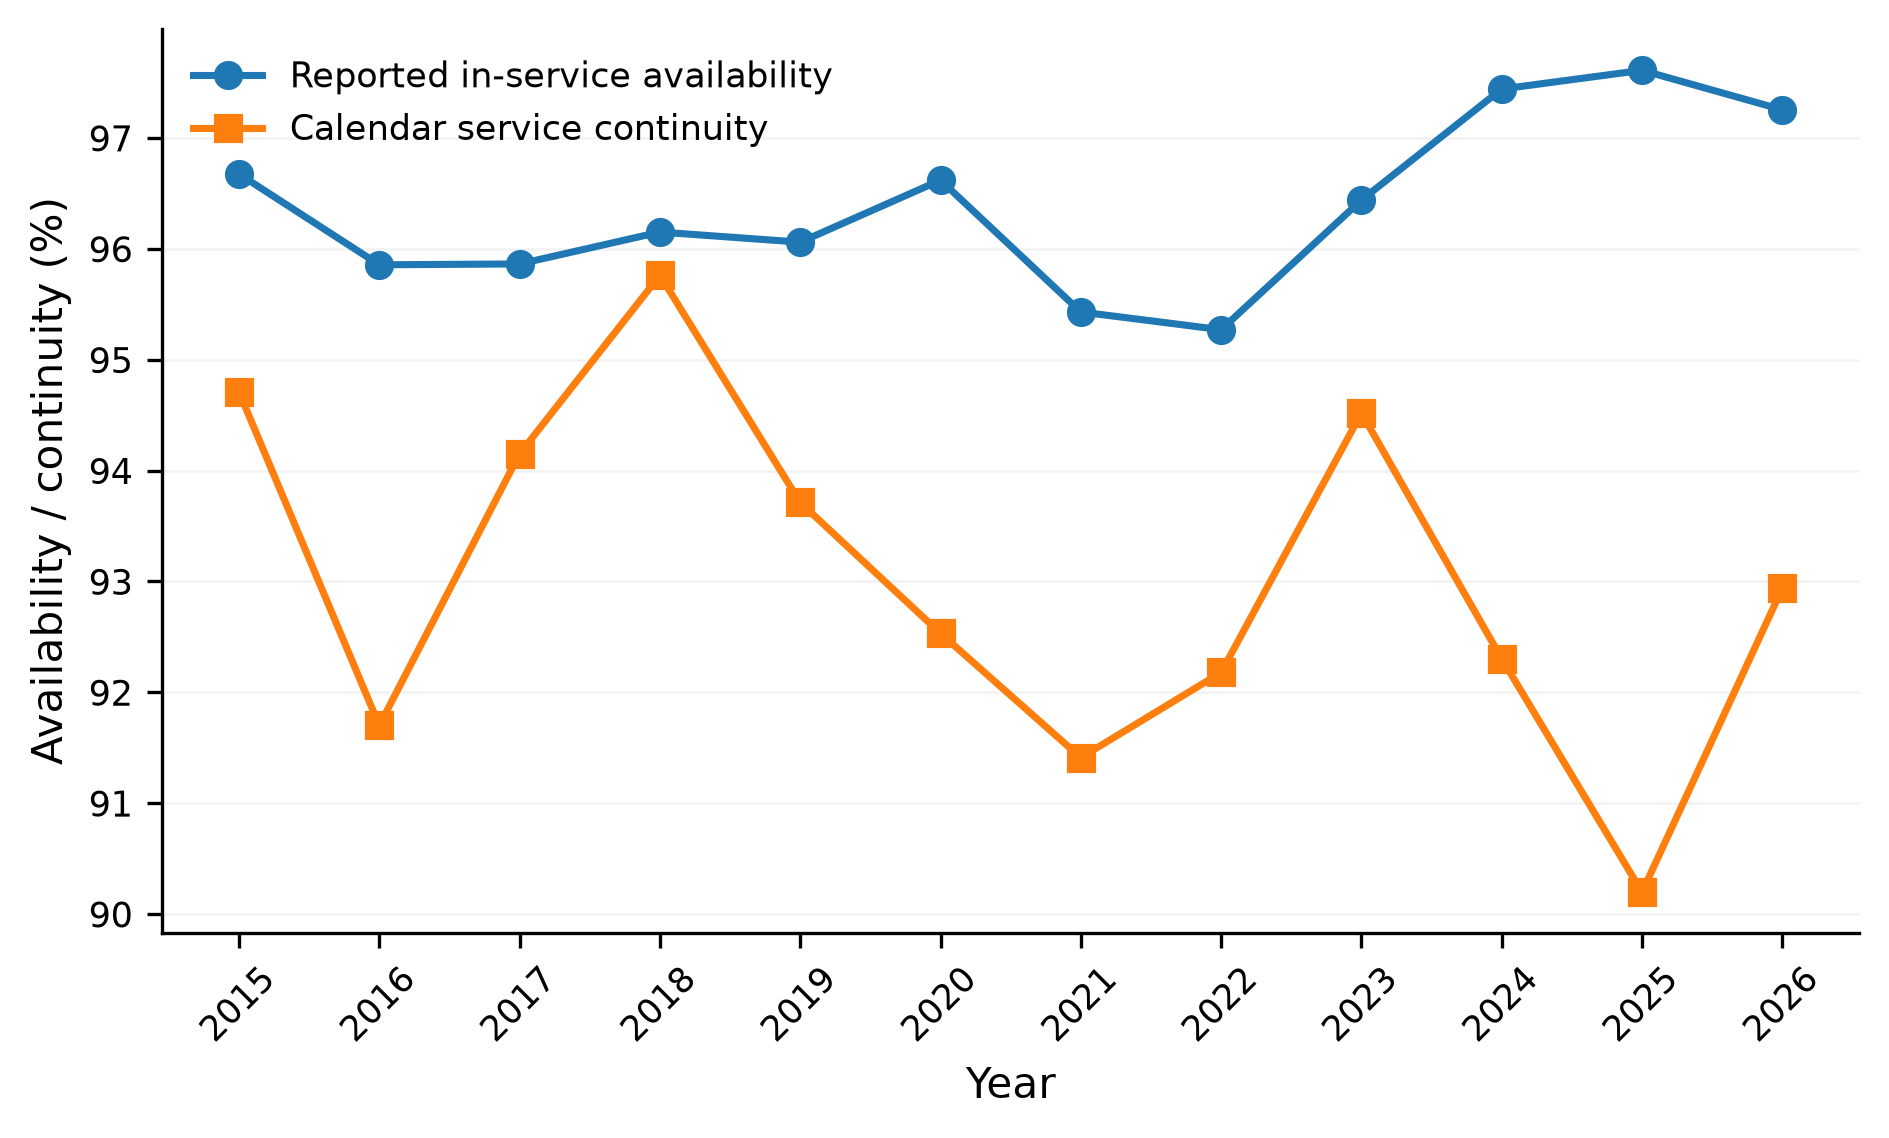
\includegraphics[width=0.92\linewidth]{fig2_metric_gap.png}
\caption{Annual MTA-reported elevator availability and calendar continuity, 2015--2026. The 2026 observation covers January--October. Annual values describe the asset composition observed in each year.}
\label{fig:trend}
\end{figure}

The 2025 gap also varied across boroughs (Table~\ref{tab:borough2025}). The Bronx combined 97.46\% MTA-reported availability with 81.70\% calendar continuity, producing a 15.77-point gap. Brooklyn and Queens also showed substantial differences, while Manhattan's gap was 5.20 points.

\begin{table}[htbp]
\centering
\caption{Borough-level elevator service measures, 2025.}
\label{tab:borough2025}
\begin{threeparttable}
\small
\begin{tabular}{lrrr}
\toprule
Borough & MTA-reported (\%) & Calendar (\%) & Gap (pp) \\
\midrule
Bronx & 97.46 & 81.70 & 15.77 \\
Brooklyn & 98.41 & 90.30 & 8.11 \\
Manhattan & 97.07 & 91.86 & 5.20 \\
Queens & 98.31 & 91.57 & 6.73 \\
\bottomrule
\end{tabular}
\begin{tablenotes}
\raggedright\footnotesize
\item The gap is MTA-reported availability minus calendar continuity.
\end{tablenotes}
\end{threeparttable}
\end{table}

The published metric is internally consistent. The difference arises because MTA-reported availability measures performance during time retained in the operator denominator, whereas calendar continuity retains the full calendar period.

\subsection{Denominator choice changes the geography of persistent low reliability}

Among the 113 station complexes with at least 36 observed months, seven fell in the lowest calendar-continuity quartile in at least half of their observed months. Figure~\ref{fig:map} maps those locations together with complexes showing a recurrence increase of at least 0.15 when calendar continuity replaces MTA-reported availability. These cut points are descriptive diagnostics rather than external service standards.

\begin{figure}[htbp]
\centering
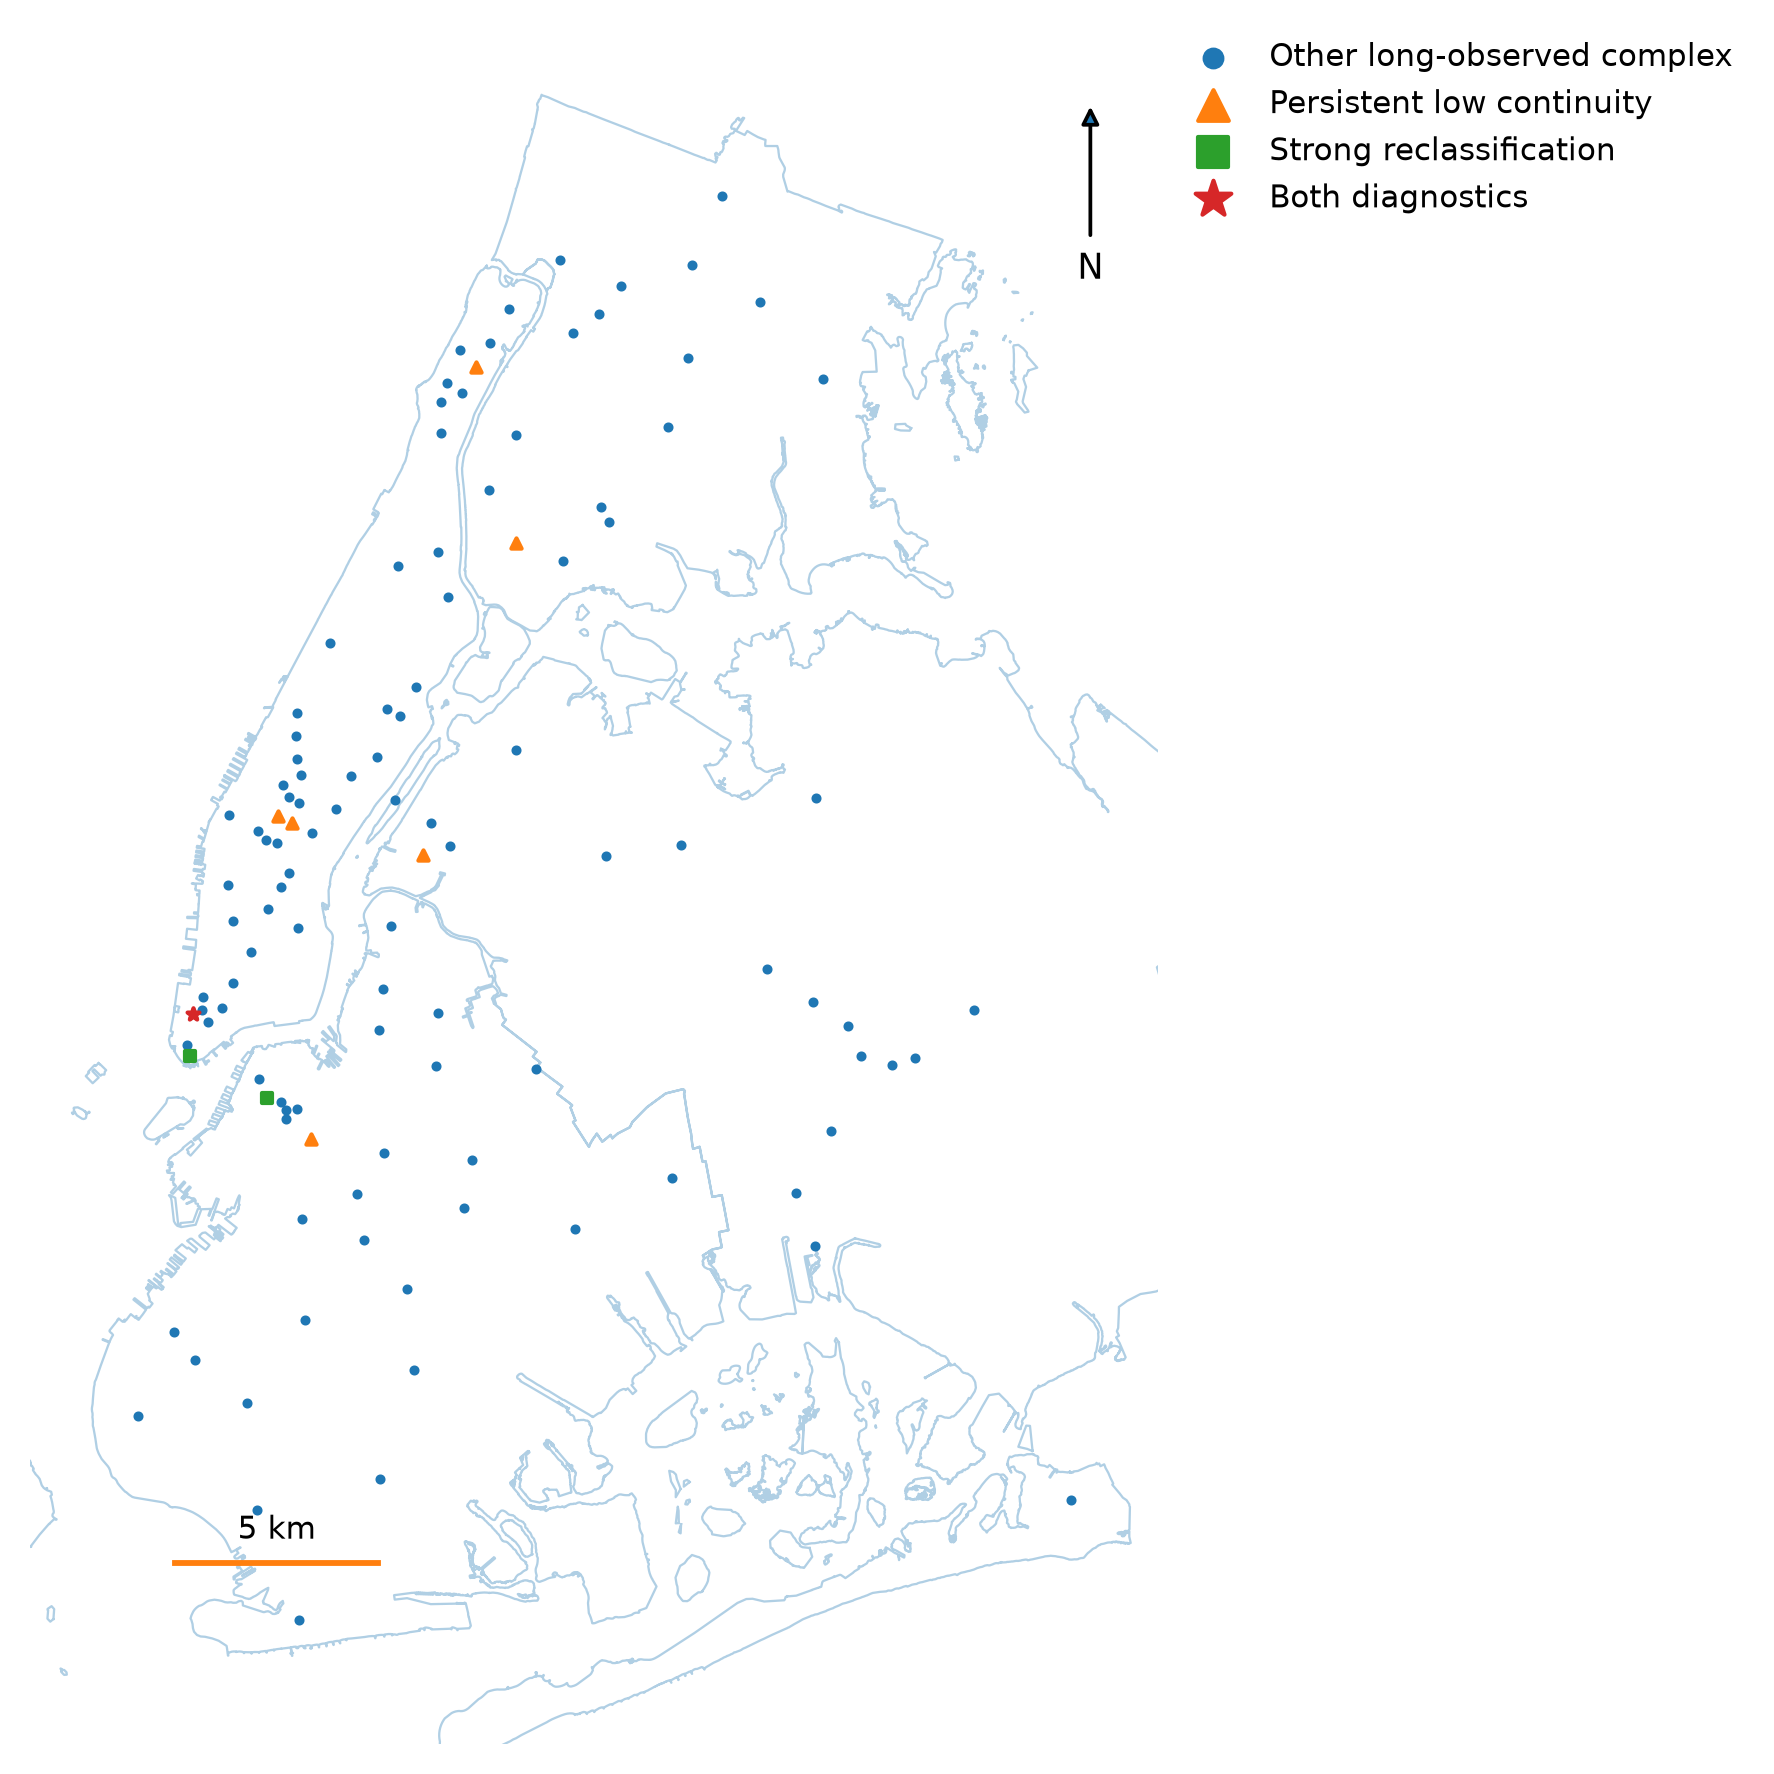
\includegraphics[width=0.88\linewidth]{fig1_spatial.png}
\caption{Spatial distribution of long-observed elevator-equipped station complexes. Symbols are mutually exclusive: persistent low continuity indicates membership in the lowest calendar-continuity quartile in at least 50\% of observed months; strong reclassification indicates an increase of at least 0.15 in low-reliability recurrence; both diagnostics indicates that both conditions are met. Station-complex coordinates are from MTA Subway Stations and Complexes, and borough boundaries are from the New York City Department of City Planning \citep{mta_stations2026,nycdcp_boroughs2026}.}
\label{fig:map}
\end{figure}

The largest reclassification occurred at Cortlandt Street (complex 328). It was in the monthly low-reliability quartile in 13.3\% of valid months under MTA-reported availability and 67.3\% under calendar continuity. South Ferry/Whitehall Street increased from 12.4\% to 29.6\%, while Court Street/Borough Hall increased from 26.1\% to 43.0\%. Figure~\ref{fig:reclass} shows the continuous recurrence difference across all eligible complexes.

\begin{figure}[htbp]
\centering
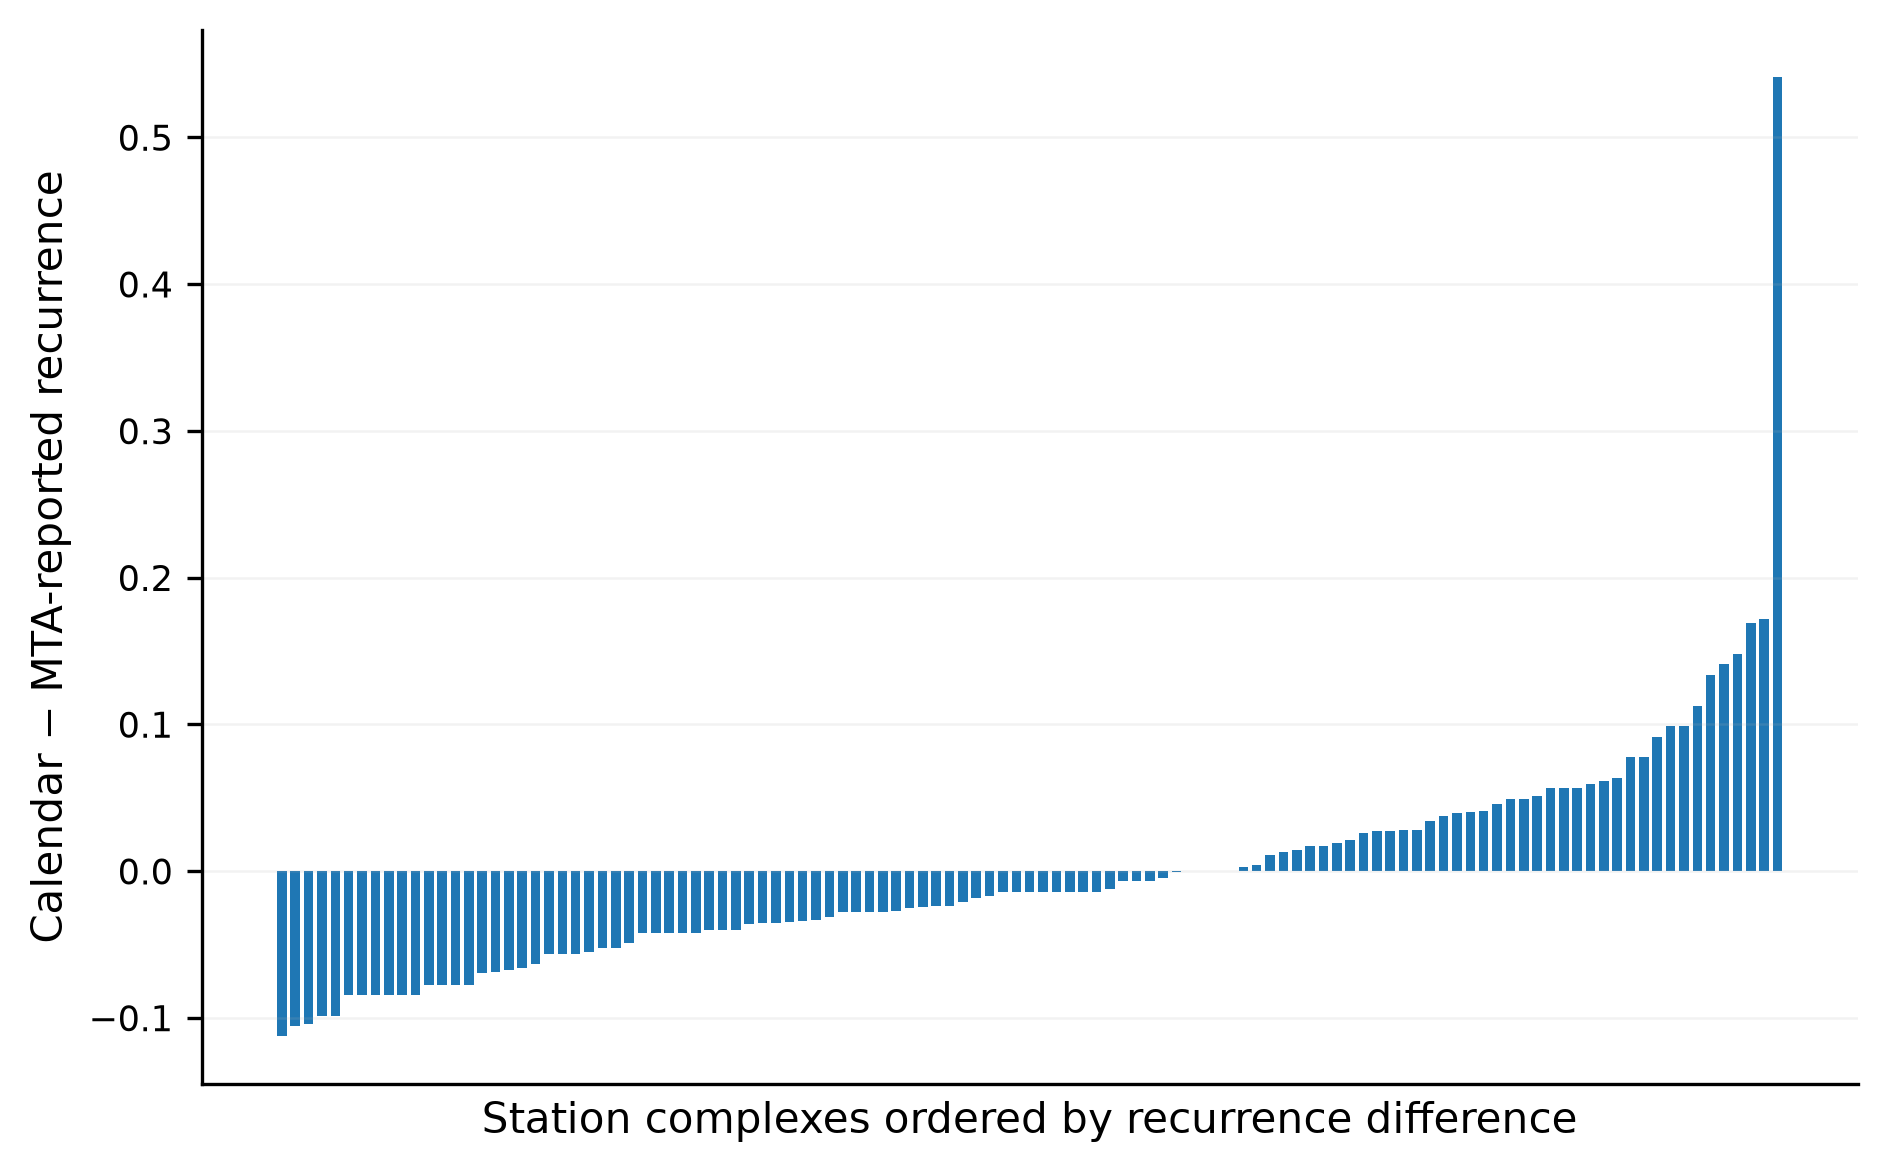
\includegraphics[width=0.72\linewidth]{fig3_reclassification.png}
\caption{Difference in station-complex low-reliability recurrence between calendar continuity and MTA-reported availability. Complexes are ordered by the recurrence difference. Positive bars indicate more frequent low-reliability classification when denominator-excluded calendar time is retained. Missing MTA-reported values are excluded from the corresponding recurrence denominator.}
\label{fig:reclass}
\end{figure}

The two recurrence measures remain strongly associated, but the relationship is not one-to-one. Under the primary 36-month and bottom-quartile specification, their Spearman correlation is 0.877. The three strongest reclassified complexes remain above the 0.15 recurrence-difference threshold when the low-reliability definition is changed to either the bottom quintile or the bottom tercile.

\subsection{Relative reliability is persistent under both service measures}

Station-complex rankings show substantial persistence from one year to the next. For MTA-reported availability, all eleven adjacent-year Spearman correlations are positive and statistically significant (Fig.~\ref{fig:persistence}). The mean is 0.562, with values from 0.405 in 2019--2020 to 0.666 in 2024--2025. Calendar continuity produces the same general pattern: the mean adjacent-year correlation is 0.525, with all eleven correlations positive and statistically significant.

\begin{figure}[htbp]
\centering
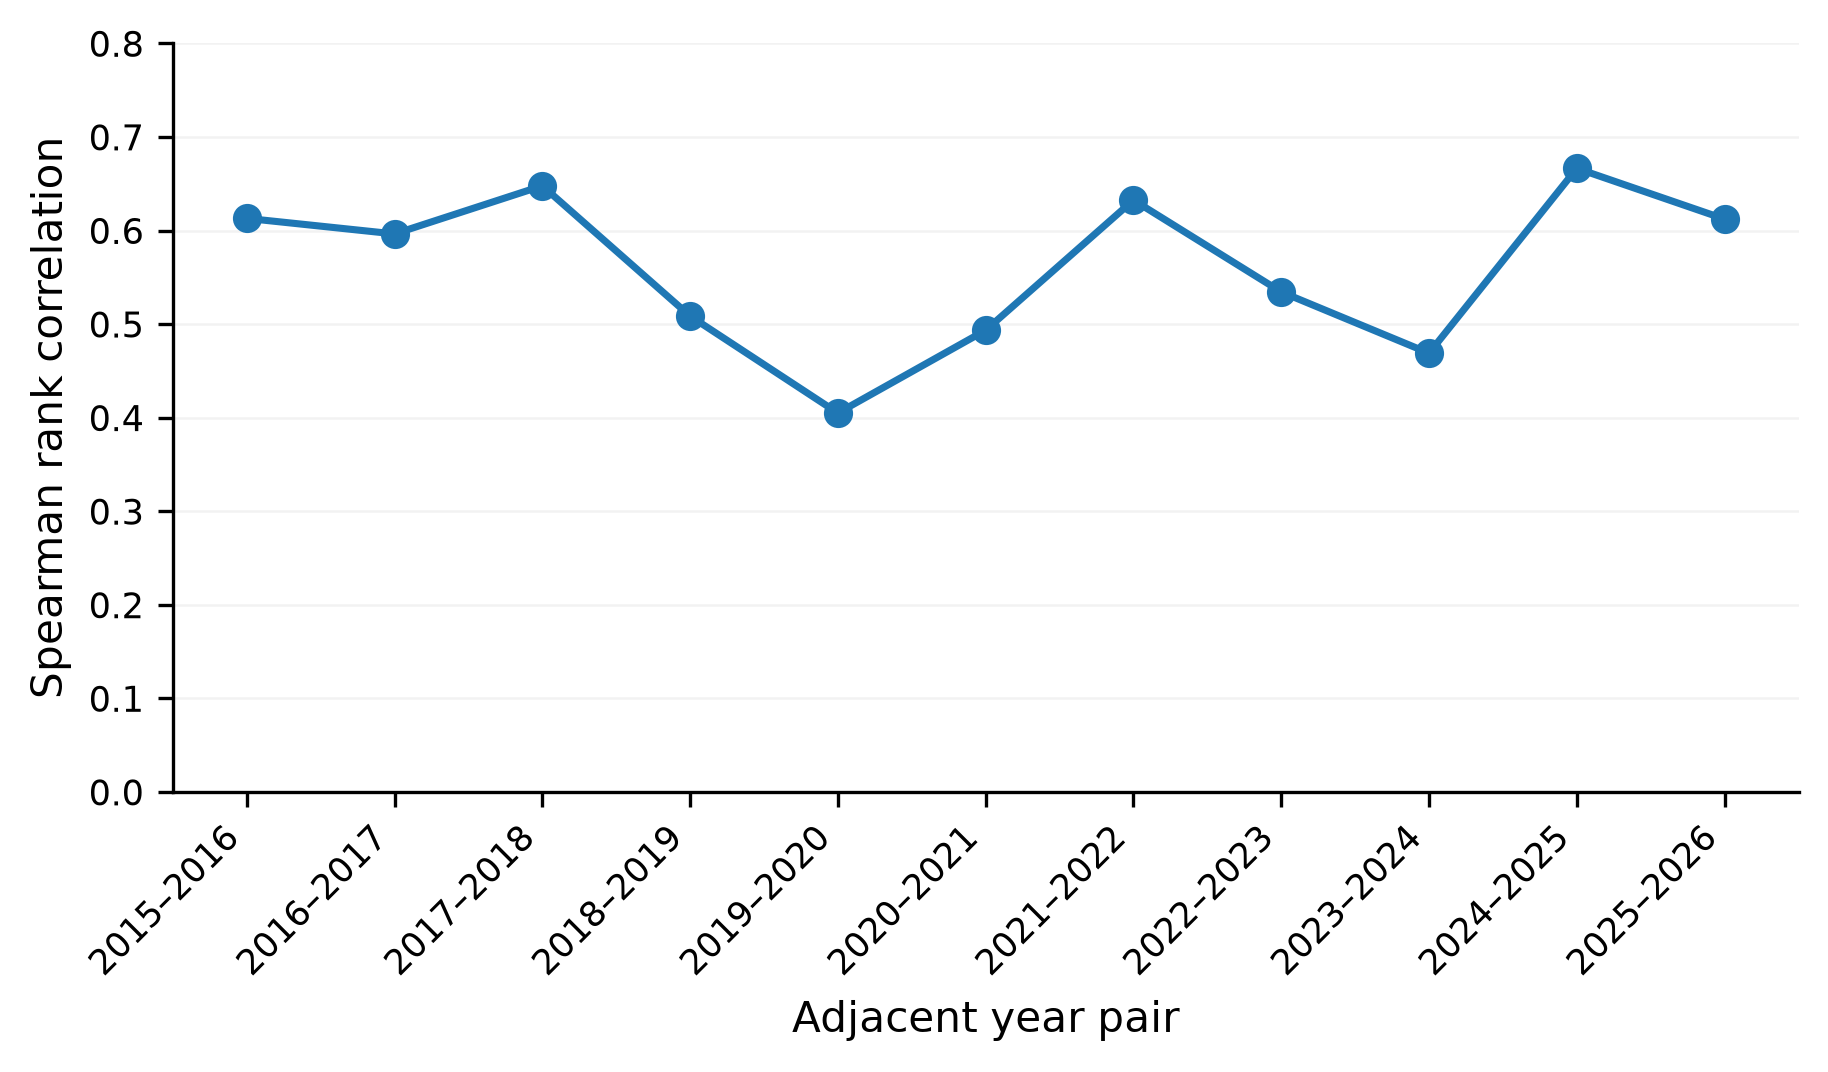
\includegraphics[width=0.92\linewidth]{fig4_persistence.png}
\caption{Spearman rank correlation of station-complex MTA-reported availability in adjacent years. Complexes must have at least six observed months in each year. The 2025--2026 pair uses January--October 2026; partial-year sensitivity results are reported in the text.}
\label{fig:persistence}
\end{figure}

The partial 2026 period does not drive the reported-availability result. Excluding the 2025--2026 pair changes the mean adjacent-year correlation from 0.562 to 0.557. When every year is restricted to January--October, the 2025--2026 correlation is 0.561 for MTA-reported availability and 0.477 for calendar continuity. Calendar-continuity persistence is shown separately in the Supplementary Material.

\subsection{Asset and platform metrics are related but spatially non-equivalent}

Across 420 borough--month observations in the overlapping 2018--2026 period, aggregated elevator MTA-reported availability and accessible-platform availability have a Spearman correlation of 0.697 and a mean absolute difference of 1.23 percentage points. Numerical association does not translate into stable spatial ordering. The complete four-borough ranking is identical in 11 of 105 complete months (10.5\%), and 64.5\% of borough rank positions change between the two measures.

Figure~\ref{fig:comparison} shows the month-by-month Kendall concordance of the four-borough rankings. The mean Kendall coefficient is 0.286, indicating that agreement in relative borough order varies substantially through time.

\begin{figure}[htbp]
\centering
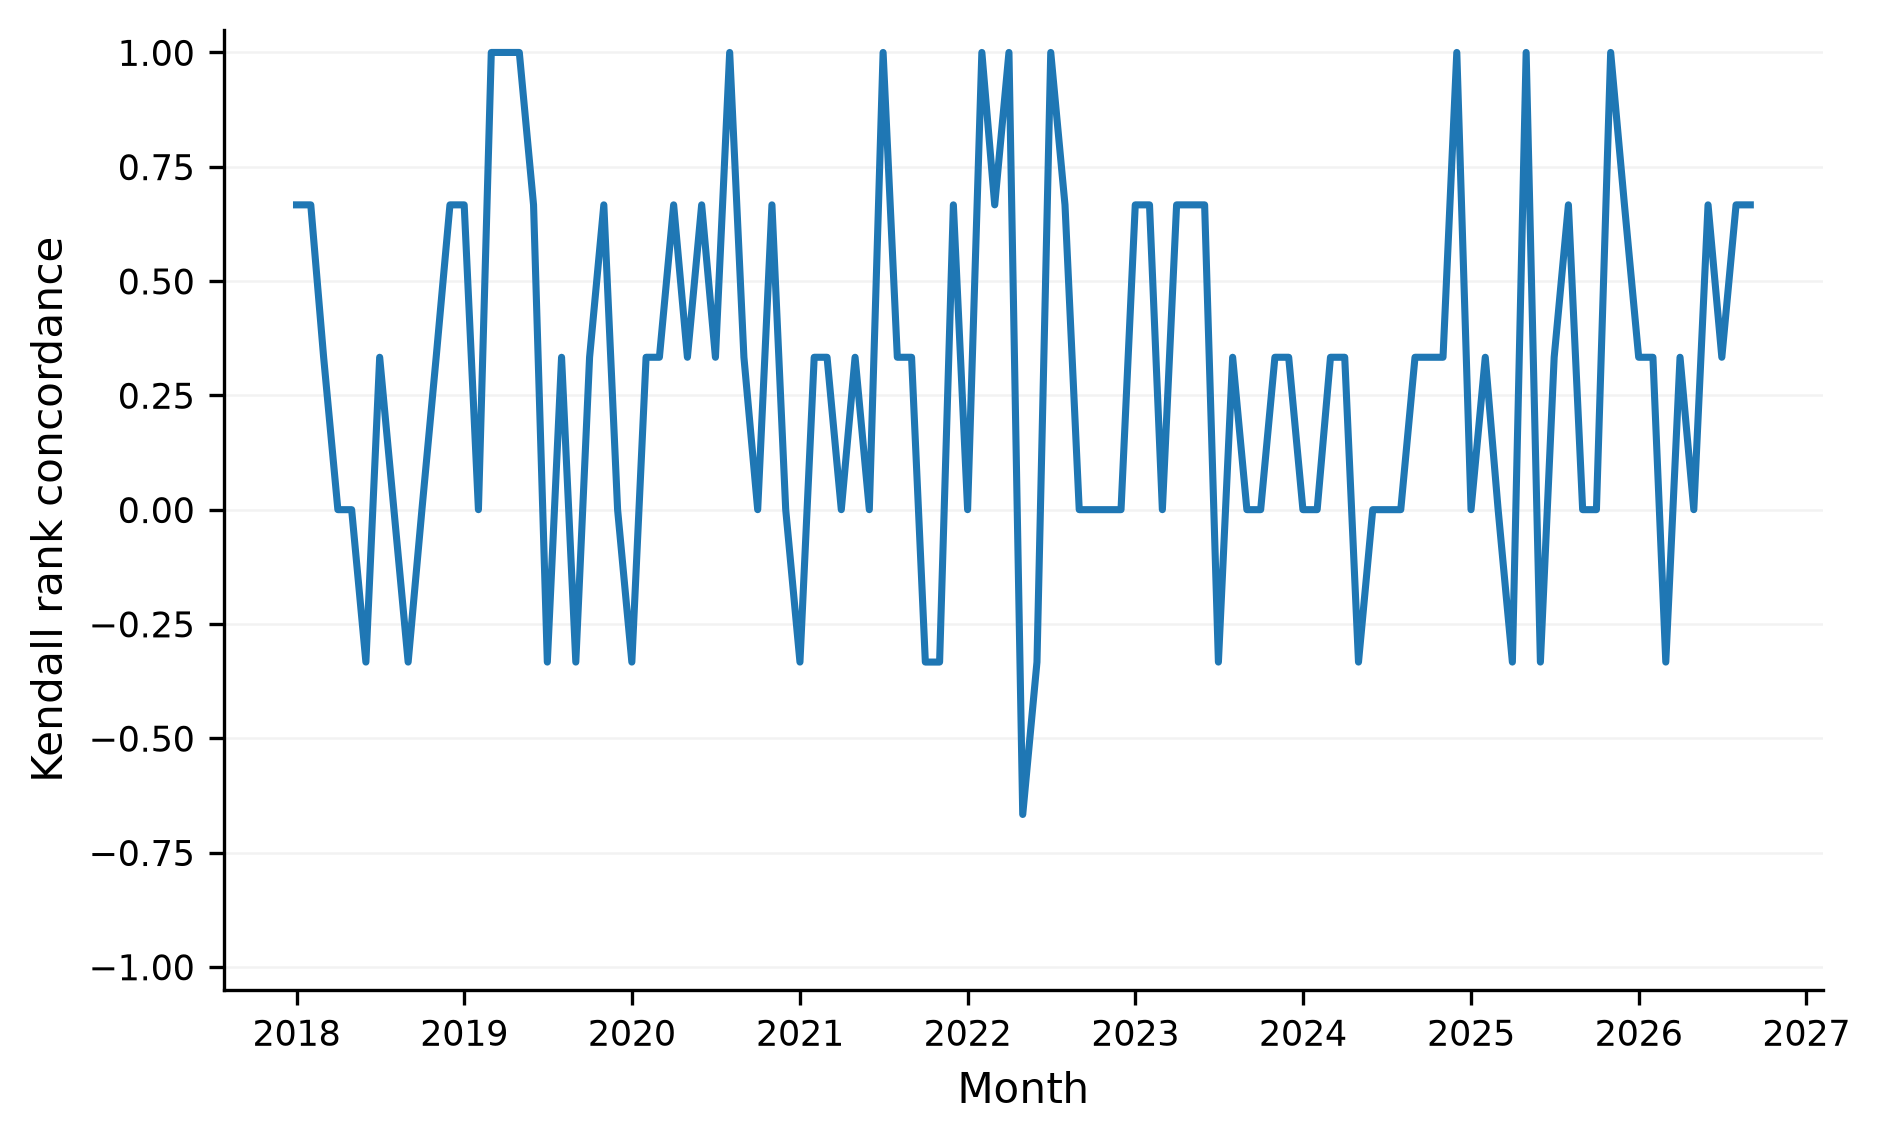
\includegraphics[width=0.92\linewidth]{fig5_concordance.png}
\caption{Monthly Kendall rank concordance between borough rankings derived from aggregated elevator MTA-reported availability and MTA accessible-platform availability, 2018--2026. A value of 1 indicates identical borough ordering.}
\label{fig:comparison}
\end{figure}

The two indicators operate at different spatial and functional levels. The comparison therefore shows concordance rather than validation: asset reliability and accessible-platform availability are related, yet they frequently prioritise boroughs differently.

\subsection{Sensitivity analyses support the measurement interpretation}

The 2025 calendar-time decomposition clarifies the source of the headline gap. Across all elevator records, 90.20\% of calendar hours were recorded as available. A further 2.21\% were unavailable within the MTA-reported denominator, while 7.59\% were excluded from that denominator. Excluded time therefore accounted for 77.5\% of total calendar service loss in 2025.

The borough pattern was concentrated rather than uniform within each borough. In the Bronx, excluded time represented 88.4\% of total calendar service loss, but 96.9\% of Bronx excluded hours came from the three station complexes with the largest excluded-hour totals. The single largest complex accounted for 63.3\%. The large Bronx gap should therefore be read as a borough-level concentration of specific station-complex conditions rather than a uniform borough-wide service state.

Removing the first and last observed month of every elevator changed 2025 systemwide calendar continuity from 90.20\% to 90.29\%. The longitudinal-coverage sensitivity is similarly stable. When the minimum observation requirement is varied from 24 to 72 months, the Spearman association between the two chronicity measures ranges from 0.863 to 0.877; seven complexes remain below the calendar-continuity quartile in at least half of their observed months, and three retain recurrence increases of at least 0.15.

Changing the descriptive low-reliability cut point also preserves the main reclassification pattern. Across bottom-quintile, quartile, and tercile definitions, the correlation between MTA-reported and calendar-continuity recurrence ranges from 0.814 to 0.906. Cortlandt Street, South Ferry/Whitehall Street, and Court Street/Borough Hall exceed a 0.15 recurrence increase under all three definitions.

Network expansion does not account for the measurement gap. A common-asset sensitivity panel contains 260 elevators observed for at least ten months in every year from 2015 through 2025. In that stable panel, the 2025 gap is 10.99 percentage points, compared with 7.41 points in the full 2025 system. The annual series in Fig.~\ref{fig:trend} is therefore descriptive of each year's system composition, while the denominator effect remains substantial under a fixed asset set.

\section{Discussion}

\subsection{The spatial consequence of a reliability denominator}

The main result is straightforward: a high operational availability percentage does not uniquely describe the continuity of accessible transport service. Reported elevator availability and calendar service continuity are both valid for their intended questions, but they encode different treatment of time. When excluded periods are spatially uneven, metric choice becomes a transport-geographical issue because it changes the places identified as persistently disadvantaged. This finding is consistent with a wider turn in accessibility research toward testing what an indicator actually represents. Recent JTG work shows that alternative measurement frameworks can expose service deficits hidden by conventional accessibility scores \citep{schroth2026}, while reviews of perceived accessibility similarly document mismatches between calculated indicators and the accessibility experienced or perceived by users \citep{negm2025}. Our result operates at a narrower infrastructure layer, but the methodological implication is the same: conclusions about spatial disadvantage depend on the measurement construct.

This extends the broader literature on scheduled versus realised accessibility. \citet{liu2024} and \citet{nichols2024} show that disruptions and recurring delays can reduce the accessibility that public transport actually delivers relative to timetable-based expectations. \citet{braga2026} shows that travel-time variability can change inequality estimates. Our results identify an analogous issue at the infrastructure layer. The gap does not arise from timetable uncertainty; it arises from how operational time is counted for vertical access assets. Yet the spatial implication is similar: a supply-side metric that is appropriate for one monitoring purpose can understate the burden relevant to another.

The 2025 Bronx result illustrates this point. Reported elevator availability remained above 97\%, which by itself suggests a highly reliable service. Calendar continuity was about 82\%. A passenger-facing interpretation of the system should not collapse these two numbers into one. The first indicates that elevators performed well during the time included in the availability denominator. The second indicates that a larger share of calendar time was not available for elevator service. For spatial service diagnosis, both are relevant; linking those service differences to population exposure is a subsequent equity question.

\subsection{Persistent places rather than isolated failures}

The adjacent-year correlations add a second dimension. Reliability disadvantage persists. That does not mean the same stations are always worst, nor does it identify a single mechanism. It does mean that repeated low ranking is common enough to be geographically structured.

This distinction matters for intervention. An occasional outage can be treated as a systemwide maintenance risk. A station complex that repeatedly falls into the low-reliability tail requires a place-based explanation. Possible mechanisms include asset age, station complexity, replacement programmes, exposure to weather, ownership, and maintenance responsibility. The management results indicate that governance should be part of that explanation, although the present analysis cannot isolate a causal effect.

The reclassification results are also important for prioritisation. Cortlandt Street looks relatively unproblematic under the published availability ranking but becomes a persistent low-continuity location when calendar exclusions are retained. In a monitoring system that uses only the reported rate, such a location is less likely to be identified as a chronic reliability concern. This is precisely the type of ``spatial so what'' that a transport-geographical analysis needs: the measurement convention changes the geography of the policy problem.

\subsection{Implications for accessible transport monitoring}

The practical implication is not to replace existing reliability KPIs. Operators need conditional reliability indicators because maintenance teams need to know how equipment performs while in operational service. A separate continuity indicator would answer a complementary question: how consistently can users expect the asset to be available over calendar time?

A two-indicator reporting framework could therefore separate \emph{in-service reliability} from \emph{service continuity}. The first would retain the operator's existing denominator. The second would explicitly count long replacement and other excluded periods. Reporting both at station or station-complex level would make spatial persistence visible and would reduce the risk that a high systemwide average obscures concentrated local service loss.

For people with mobility disabilities, this distinction has a direct accessibility meaning. \citet{liu2023} demonstrates that transit accessibility and usage already differ substantially for mobility-disabled travellers. \citet{arai2026} shows that formal elevator provision does not eliminate additional within-station travel burdens. Our findings add a temporal dimension: even where vertical access exists, the continuity of that access varies across places and time.

\subsection{Why the platform comparison matters}

The comparison with accessible-platform availability provides a useful external check. The moderate-to-strong correlation confirms that equipment reliability is related to higher-level step-free service. The frequent ranking disagreement shows why asset-level results should not be interpreted as a direct substitute for passenger accessibility.

This difference strengthens, rather than weakens, the measurement argument. Public transport accessibility is multi-layered. Asset condition, platform availability, network connectivity, service reliability, and passenger destinations operate at different spatial and functional scales. A single KPI cannot represent all of them. The analytical task is therefore to match the metric to the question and to test whether conclusions are stable when the scale or denominator changes.

\section{Limitations}

Four limitations define the scope of the findings. First, calendar continuity treats all calendar hours outside the reported denominator as unavailable asset service. This is appropriate for a sensitivity analysis of continuous asset provision, but it does not reveal why the time was excluded. Planned replacement, major capital work, temporary alternative arrangements, and other states may have different passenger implications.

Second, the analysis is conducted at equipment and station-complex levels. It does not reconstruct complete street-to-platform vertical paths or origin--destination journeys. An unavailable elevator can be redundant at one station and a single point of failure at another. The results therefore concern the geography of elevator service continuity, not the probability that an individual trip is step-free.

Third, the management analysis is observational. Complex and month fixed effects remove substantial spatial and temporal confounding, and the mixed-management sensitivity analysis gives a similar estimate, but management responsibility is not randomly assigned.

Fourth, the platform availability comparison is aggregated to borough level because that is the granularity of the published historical indicator. Future work could combine the continuity measure with station-level path redundancy, passenger flows, and contemporaneous outage logs to estimate passenger-weighted consequences while preserving the distinction between capital replacement and routine reliability.

\section{Conclusions}

This paper asks a simple transport-geographical question: does the way elevator reliability is measured change where accessible transport service appears unreliable? Using 46,400 monthly elevator records from the New York City subway, the answer is yes.

Reported in-service availability was consistently higher than calendar service continuity, and the gap was strongly uneven across years and boroughs. In 2025, the systemwide difference was 7.41 percentage points and reached 15.77 points in the Bronx. Station-complex rankings also showed substantial year-to-year persistence, indicating that low reliability is geographically structured rather than entirely episodic. For several complexes, retaining denominator-excluded time substantially increased the frequency with which they were identified as chronically low-reliability places. Third-party management was associated with lower reported availability even within station-complex and month controls. Finally, asset and platform metrics were correlated but rarely produced the same spatial ordering of boroughs.

The wider implication is methodological. Accessibility monitoring should distinguish the reliability of infrastructure while it is counted as in service from the continuity of the service available to travellers over time. When those denominators differ systematically across space, measurement becomes part of the geography of transport service disadvantage.

\section*{Data availability}

The two primary datasets are publicly available from New York State Open Data through the Metropolitan Transportation Authority. Reproducible processing and figure-generation code will be archived with the manuscript repository. The analysis uses a frozen data snapshot downloaded on 16 November 2026; the repository workflow is designed to retrieve newer official releases separately so that the submitted results remain reproducible.



\section*{Declaration of generative AI and AI-assisted technologies in the writing process}
During the preparation of this work, the author(s) used OpenAI ChatGPT to assist with drafting and debugging analysis code, manuscript organization, and language editing. After using this tool, the author(s) reviewed and verified the code, statistical outputs, references, and manuscript content as needed and take(s) full responsibility for the content of the publication.

\bibliographystyle{elsarticle-harv}
\bibliography{references}
\end{document}
